\documentclass[12pt,a4paper]{article}

\usepackage[x11names]{xcolor}
\usepackage{pgfplots}
\pgfplotsset{compat=1.16}


\colorlet{covercolor}{LightPink1}
\colorlet{bookcolor}{LightPink4}
\colorlet{chapnumcolor}{LightPink3}
\colorlet{listingnumbercolor}{bookcolor}
\colorlet{listingbgcolor}{LightPink1!30!white}
\colorlet{infoboxbg}{LightPink1!30!white}
\colorlet{infoboxbgtitle}{LightPink1}


\begin{document}

\begin{figure}[!ht]
\centering
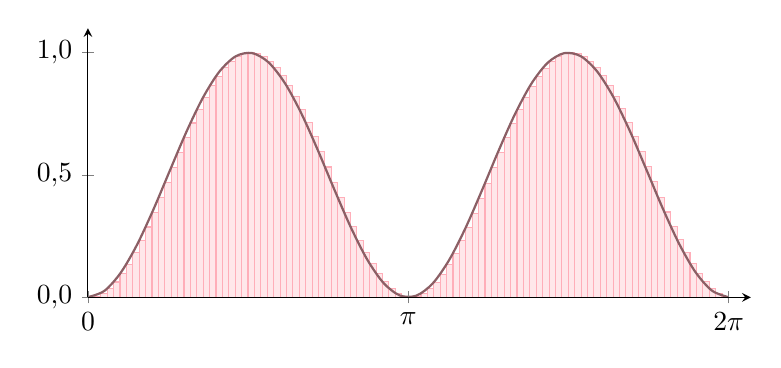
\begin{tikzpicture}[
  declare function = { f(\x) = sin(deg(\x))^2; }
]
\begin{axis}[width=10cm, height=5cm,
   tick label style = {
      /pgf/number format/use comma,
      /pgf/number format/fixed,
      /pgf/number format/fixed zerofill,
      /pgf/number format/precision = 1},
    xtick={0,pi,2*pi},
    xticklabels={$0$,$\pi$,$2\pi$},
    ytick={0,0.5,1.0},
    xmax=6.5,ymax=1.1,ymin=-0.001,xmin=-0.0,
%    enlargelimits=true,
    axis y line=middle, axis x line=bottom,
    clip=false,
    domain=0:17,
    axis on top
    ]

\addplot [draw=covercolor, fill=infoboxbg, ybar interval, samples=101, domain=0:6.28] {f(x)} \closedcycle;

\addplot[smooth, thick,domain=0:6.28,samples=40,draw=bookcolor]{f(x)};

\end{axis}
\end{tikzpicture}
\end{figure}

Oppervlakte $O$ onder de functie:

\begin{equation}
O = \int_{a}^{b}f(x)\,\mathrm{d}x = \lim\limits_{n\to\infty}\sum_{k=0}^{n-1}f\left(a+k\frac{b-a}{n}\right)\cdot\frac{b-a}{n}
\end{equation}

\end{document}